\documentclass[twoside,11pt]{article}
\usepackage[T1]{fontenc}

% Any additional packages needed should be included after jmlr2e.
% Note that jmlr2e.sty includes epsfig, amssymb, natbib and graphicx,
% and defines many common macros, such as 'proof' and 'example'.
%
% It also sets the bibliographystyle to plainnat; for more information on
% natbib citation styles, see the natbib documentation, a copy of which
% is archived at http://www.jmlr.org/format/natbib.pdf

\usepackage{jmlr2e}
\usepackage{amsmath}
\usepackage{amsfonts}
\usepackage{amssymb}
\usepackage{mathtools}
\usepackage{booktabs}
\usepackage{bbold}
\usepackage{thm-restate}
\usepackage{caption}
\usepackage{subfig}
%\usepackage{bbold}
\usepackage[ruled,linesnumbered,lined,commentsnumbered]{algorithm2e}
\usepackage[colorinlistoftodos, textwidth=22mm, shadow]{todonotes}
\definecolor{blued}{RGB}{70,197,221}
\definecolor{pearOne}{HTML}{2C3E50}
%A9CF54
\definecolor{pearTwo}{HTML}{A9CF54}
\definecolor{pearTwoT}{HTML}{C2895B}
\definecolor{pearThree}{HTML}{FF69B4}
\colorlet{titleTh}{pearOne}
\colorlet{bull}{pearTwo}
\definecolor{pearcomp}{HTML}{B97E29}
\definecolor{pearFour}{HTML}{588F27}
\definecolor{pearFith}{HTML}{ECF0F1}
\definecolor{pearDark}{HTML}{2980B9}
\definecolor{pearDarker}{HTML}{F330DB}
\hypersetup{
	colorlinks,
	citecolor=pearDark,
	linkcolor=pearThree,
	urlcolor=pearDarker}

% Definitions of handy macros can go here

\newcommand{\dataset}{{\cal D}}
\newcommand{\fracpartial}[2]{\frac{\partial #1}{\partial  #2}}

%\DeclareMathOperator*{\argmin}{arg\,min}
%\DeclareMathOperator*{\argmax}{arg\,max}
%\DeclarePairedDelimiter{\ceil}{\lceil}{\rceil}

%%% todos
%\usepackage[colorinlistoftodos, textwidth=30mm, shadow, textsize=small]{todonotes}
%\definecolor{babyblue}{rgb}{0.54, 0.81, 0.94}
%\definecolor{citrine}{rgb}{0.89, 0.82, 0.04}
%\definecolor{misocolor}{rgb}{0.16,0.27,0.86}
%\newcommand{\todom}[1]{\todo[color=misocolor!30]{#1}\xspace}
%\newcommand{\todomi}[1]{\todo[inline,color=misocolor!30]{#1}}

\definecolor{graphicbackground}{rgb}{0.96,0.96,0.8}
\definecolor{rouge1}{RGB}{226,0,38}  % red P
\definecolor{orange1}{RGB}{243,154,38}  % orange P
\definecolor{jaune}{RGB}{254,205,27}  % jaune P
\definecolor{blanc}{RGB}{255,255,255} % blanc P
\definecolor{rouge2}{RGB}{230,68,57}  % red S
\definecolor{orange2}{RGB}{236,117,40}  % orange S
\definecolor{taupe}{RGB}{134,113,127} % taupe S
\definecolor{gris}{RGB}{91,94,111} % gris S
\definecolor{bleu1}{RGB}{38,109,131} % bleu S
\definecolor{bleu2}{RGB}{28,50,114} % bleu S
\definecolor{vert1}{RGB}{133,146,66} % vert S
\definecolor{vert3}{RGB}{20,200,66} % vert S
\definecolor{vert2}{RGB}{157,193,7} % vert S
\definecolor{darkyellow}{RGB}{233,165,0}  % orange S
\definecolor{lightgray}{rgb}{0.9,0.9,0.9}
\definecolor{darkgray}{rgb}{0.6,0.6,0.6}
\definecolor{babyblue}{rgb}{0.54, 0.81, 0.94}
\definecolor{citrine}{rgb}{0.89, 0.82, 0.04}
\definecolor{misogreen}{rgb}{0.25,0.6,0.0}

\newcommand{\rcol}[1]{\textcolor{red}{\textit{#1}}}
\newcommand{\defcol}[1]{\textcolor{vert3}{\textbf{#1}}}
\newcommand{\yellcol}[1]{\textcolor{babyblue}{\textbf{#1}}}
\newcommand{\gcol}[1]{\textcolor{vert3}{\textbf{#1}}}

\newcommand{\emphcol}[1]{\textcolor{vert3}{\textbf{#1}}}

\newcommand{\grcol}[1]{\textcolor{gray}{#1}}
\newcommand{\notecol}[1]{\textcolor{gray}{#1}}

\newcommand{\bcol}[1]{\textcolor{blue}{\textit{#1}}}
\newcommand{\ycol}[1]{\textcolor{darkyellow}{\textit{#1}}}
\newcommand{\rcolb}[1]{\textcolor{red}{\textit{\textbf{#1}}}}
\newcommand{\gcolb}[1]{\textcolor{vert3}{\textit{\textbf{#1}}}}
\newcommand{\bcolb}[1]{\textcolor{blue}{\textit{\textbf{#1}}}}
\newcommand{\ycolb}[1]{\textcolor{darkyellow}{\textit{\textbf{#1}}}}
\newcommand{\mcolA}[1]{{\color{bleu1} #1}}
\newcommand{\mcolB}[1]{{\color{darkyellow} #1}}
\newcommand{\mcolC}[1]{{\color{misogreen} #1}}


\DeclareMathOperator*{\argmax}{arg\,max}
\DeclareMathOperator*{\argmin}{arg\,min}
\DeclareMathOperator*{\arginf}{arg\,inf}
\DeclareMathOperator*{\sgn}{sgn}
%\DeclareMathOperator{\regret}{regret}
\DeclareMathOperator{\polylog}{polylog}
\DeclareMathOperator{\logloglog}{logloglog}
\DeclareMathOperator{\polyloglog}{polyloglog}


\newcommand*\diff{\mathop{}\!\mathrm{d}}
\newcommand*\Diff[1]{\mathop{}\!\mathrm{d^#1}}
\renewcommand{\d}[1]{\ensuremath{\operatorname{d}\!{#1}}}

\newcommand{\set}[1]{\left\{#1\right\}}
%\DeclarePairedDelimiter\ceil{\lceil}{\rceil}
%\DeclarePairedDelimiter\floor{\lfloor}{\rfloor}
\newcommand{\ceil}[1]{\left\lceil#1\right\rceil}
\newcommand{\floor}[1]{\left\lfloor#1\right\rfloor}

%\newcommand{\ceil}[1]{\lceil#1\rceil}

\newcommand{\II}[1]{\mathds{1}_{\left\{#1\right\}}}
\newcommand{\I}{{\mathds{1}}}


%arrows
\newcommand{\ra}{\rightarrow}

%distributions
\newcommand{\Bernoulli}{\mathrm{Bernoulli}}


\newcommand{\specialcell}[2][c]{%
 \begin{tabular}[#1]{@{}c@{}}#2\end{tabular}}

%\newtheorem{assumption}{Assumption}
%\newtheorem{lemma}{Lemma}
%\newtheorem{theorem}{Theorem}
%\newtheorem{definition}{Definition}
%\newtheorem{corollary}{Corollary}
%\newtheorem{remark}{Remark}


% \newcommand{\R}{I\!\! R}
\newcommand{\R}{\mathbb{R}}
\newcommand{\realset}{\mathbb{R}}

\newcommand{\NN}{{\mathbb N}}
\newcommand{\1}{\mathds{1}}
\newcommand{\bOne}{{\bf 1}}
\newcommand{\bZero}{{\bf 0}}
\newcommand{\E}{\mathbb{E}}
\newcommand{\EE}[1]{\mathbb{E}\left[#1\right]}
\newcommand{\EEt}[1]{\mathbb{E}_t\left[#1\right]}
\newcommand{\EEs}[2]{\mathbb{E}_{#1}\left[#2\right]}
\newcommand{\EEc}[2]{\mathbb{E}\left[#1\left|#2\right.\right]}
\newcommand{\EEcc}[2]{\mathbb{E}\left[\left.#1\right|#2\right]}
\newcommand{\EEcct}[2]{\mathbb{E}_t\left[\left.#1\right|#2\right]}
\newcommand{\PP}[1]{\mathbb{P}\left[#1\right]}
\newcommand{\PPt}[1]{\mathbb{P}_t\left[#1\right]}
 \newcommand{\PPc}[2]{\mathbb{P}\left[#1\left|#2\right.\right]}
\newcommand{\PPcc}[2]{\mathbb{P}\left[\left.#1\right|#2\right]}
\newcommand{\PPct}[2]{\mathbb{P}_t\left[#1\left|#2\right.\right]}
\newcommand{\PPcct}[2]{\mathbb{P}_t\left[\left.#1\right|#2\right]}
%parens
\newcommand{\pa}[1]{\left(#1\right)}
\newcommand{\sqpa}[1]{\left[#1\right]}
\newcommand{\ac}[1]{\left\{#1\right\}}
\newcommand{\ev}[1]{\left\{#1\right\}}
\newcommand{\card}[1]{\left|#1\right|}


\newcommand{\normtwo}[1]{\|#1\|_2}
\newcommand{\norm}[1]{\left\|#1\right\|}
\newcommand{\onenorm}[1]{\norm{#1}_1}
\newcommand{\infnorm}[1]{\norm{#1}_\infty}
\newcommand{\norminf}[1]{\infnorm{#1}}

\newcommand{\abs}[1]{\left|#1\right|}

\newcommand{\CommaBin}{\mathbin{\raisebox{0.5ex}{,}}}
\newcommand*{\MyDef}{\mathrm{\tiny def}}
\newcommand*{\eqdefU}{\ensuremath{\mathop{\overset{\MyDef}{=}}}}% Unscaled version
%\newcommand*{\eqdef}{\mathop{\overset{\MyDef}{\resizebox{\widthof{\eqdefU}}{\heightof{=}}{=}}}}
\newcommand*{\eqdef}{\triangleq}
%\newcommand{\eqdef}{\stackrel{{\rm def}}{=}}
%\newcommand{\eqdef}{\stackrel{{\rm \tiny def}}{=}}
\newcommand{\transpose}{^\mathsf{\scriptscriptstyle T}}

%Calligraphic Shorthands
\newcommand{\cA}{\mathcal{A}}
\newcommand{\cB}{\mathcal{B}}
\newcommand{\cC}{\mathcal{C}}
\newcommand{\cD}{\mathcal{D}}
\newcommand{\cE}{\mathcal{E}}
\newcommand{\F}{\mathcal{F}}
\newcommand{\cF}{\mathcal{F}}
\newcommand{\cG}{\mathcal{G}}
\newcommand{\cH}{\mathcal{H}}
\newcommand{\cI}{\mathcal{I}}
\newcommand{\cJ}{\mathcal{J}}
\newcommand{\cK}{\mathcal{K}}
\newcommand{\cL}{\mathcal{L}}
\newcommand{\calL}{\cL}
\newcommand{\cM}{\mathcal{M}}
\newcommand{\cN}{\mathcal{N}}
\newcommand{\cO}{\mathcal{O}}
\newcommand{\tcO}{\widetilde{\cO}}
\newcommand{\OO}{\mathcal{O}}
\newcommand{\tOO}{\wt{\OO}}
\newcommand{\cP}{\mathcal{P}}
\newcommand{\cQ}{\mathcal{Q}}
\newcommand{\cR}{\mathcal{R}}
\newcommand{\Sw}{\mathcal{S}}
\newcommand{\cS}{\mathcal{S}}
\newcommand{\cT}{\mathcal{T}}
\newcommand{\T}{\cT}
\newcommand{\cU}{\mathcal{U}}
\newcommand{\cV}{\mathcal{V}}
\newcommand{\cW}{\mathcal{W}}
\newcommand{\cX}{\mathcal{X}}
\newcommand{\X}{\cX}
\newcommand{\cY}{\mathcal{Y}}
\newcommand{\cZ}{\mathcal{Z}}

%Bolds Shorthands
\newcommand{\ba}{{\bf a}}
\newcommand{\bA}{{\bf A}}
\newcommand{\bb}{{\bf b}}
\newcommand{\bB}{{\bf B}}
\newcommand{\bc}{{\bf c}}
\newcommand{\bC}{{\bf C}}
\newcommand{\bD}{{\bf D}}
\newcommand{\bg}{{\bf g}}
\newcommand{\bG}{{\bf G}}
\newcommand{\bI}{{\bf I}}
\newcommand{\bM}{{\bf M}}
\newcommand{\bO}{\boldsymbol{O}}
\newcommand{\bp}{\boldsymbol{p}}
\newcommand{\bP}{{\bf P}}
\newcommand{\br}{{\bf r}}
\newcommand{\bR}{{\bf R}}
\newcommand{\bQ}{{\bf Q}}
\newcommand{\be}{{\bf e}}
\newcommand{\bff}{{\bf f}}
\newcommand{\bi}{{\bf i}}
\newcommand{\bk}{{\bf k}}
\newcommand{\bK}{{\bf K}}
\newcommand{\bL}{{\bf L}}
\newcommand{\bs}{{\bf s}}
\newcommand{\bq}{{\bf q}}
\newcommand{\bu}{{\bf u}}
\newcommand{\bU}{{\bf U}}
\newcommand{\bv}{{\bf v}}
\newcommand{\bV}{{\bf V}}
\newcommand{\bw}{{\bf w}}
\newcommand{\bW}{{\bf W}}
\newcommand{\by}{{\bf y}}
\newcommand{\bx}{{\bf x}}
\newcommand{\bX}{{\bf X}}
\newcommand{\bZ}{{\bf Z}}

\newcommand{\eps}{\varepsilon}
\renewcommand{\epsilon}{\varepsilon}
\renewcommand{\hat}{\widehat}
\renewcommand{\tilde}{\widetilde}
\renewcommand{\bar}{\overline}

\newcommand{\balpha}{{\boldsymbol \alpha}}
\newcommand{\talpha}{\widetilde{\alpha}}
\newcommand{\btheta}{{\boldsymbol \theta}}
\newcommand{\tTheta}{{\widetilde\Theta}}
\newcommand{\bdelta}{{\boldsymbol \delta}}
\newcommand{\bDelta}{{\boldsymbol \Delta}}
\newcommand{\bLambda}{{\boldsymbol \Lambda}}
\newcommand{\bSigma}{{\boldsymbol \Sigma}}
\newcommand{\bmu}{{\boldsymbol \mu}}
\newcommand{\bxi}{{\boldsymbol \xi}}
%\newcommand{\bell}{\boldsymbol \ell}

\newcommand{\nothere}[1]{}
\newcommand{\moveb}{\\ \bigskip}
\newcommand{\movebb}{\\[-0.25em]}
\newcommand{\moves}{\\ \smallskip}
\newcommand{\movess}{\\[-0.5em]}
\newcommand{\movesss}{\smallskip}

% bandits
\newcommand{\hloss}{\hat\ell}
\newcommand{\bloss}{\boldsymbol  \ell}
\newcommand{\hbl}{\hat{\bloss}}
\newcommand{\hbL}{\wh{\bL}}
\newcommand{\wh}{\widehat}
\newcommand{\ti}{_{t,i}}
\newcommand{\wt}{\widetilde}



%% from single papers, but merged here
% algo names
\usepackage{xspace}
\renewcommand{\ttdefault}{lmtt}
%stochastic bandits
\newcommand{\UCB}{\texttt{UCB}\xspace}
\newcommand{\UCBOne}{\texttt{UCB1}\xspace}
\newcommand{\UCBTwo}{\texttt{UCB2}\xspace}
\newcommand{\KLUCB}{\texttt{KL-UCB}\xspace}
%adversarial bandits
\newcommand{\MOSS}{\texttt{MOSS}\xspace}
\newcommand{\EXP}{\texttt{Exp3}\xspace}
%best arm identification
\newcommand{\Racing}{\texttt{Racing}\xspace}
\newcommand{\LUCB}{\texttt{LUCB}\xspace}
\newcommand{\KLRacing}{\texttt{KL-Racing}\xspace}
\newcommand{\KLLUCB}{\texttt{KL-LUCB}\xspace}
\newcommand{\Track}{\texttt{Track-and-Stop}\xspace}
\newcommand{\UCBE}{\texttt{UCB-E}\xspace}
\newcommand{\SR}{\texttt{SuccessiveReject}\xspace}
\newcommand{\SHA}{\texttt{SequentialHalving}\xspace}
\newcommand{\UGapE}{\texttt{UGapE}\xspace}
\newcommand{\TTTS}{\texttt{TTTS}\xspace}
\newcommand{\TTPS}{\texttt{TTPS}\xspace}
\newcommand{\TTVS}{\texttt{TTVS}\xspace}
%contextual bandits
\newcommand{\LinUCB}{\texttt{LinUCB}\xspace}
\newcommand{\LOVECON}{\texttt{ILOVETOCONBANDITS}\xspace}
\newcommand{\EpochGreedy}{\texttt{Epoch-Greedy}\xspace}
%bayesian optimization
\newcommand{\GPUCB}{\texttt{GP-UCB}\xspace}
\newcommand{\TS}{\texttt{ThompsonSampling}\xspace}
\newcommand{\EI}{\texttt{EI}\xspace}
\newcommand{\PI}{\texttt{PI}\xspace}
%continuous bandits
\newcommand{\StoSOO}{\texttt{StoSOO}\xspace}
\newcommand{\POO}{\texttt{POO}\xspace}
\newcommand{\DOO}{\texttt{DOO}\xspace}
\newcommand{\SOO}{\texttt{SOO}\xspace}
\newcommand{\Zooming}{\texttt{Zooming}\xspace}
\newcommand{\UCT}{\texttt{UCT}\xspace}
\newcommand{\HCT}{\texttt{HCT}\xspace}
\newcommand{\SHOO}{\POO}
\newcommand{\HOO}{\texttt{HOO}\xspace}
\newcommand{\ATB}{\texttt{ATB}\xspace}
\newcommand{\TZ}{\texttt{TaxonomyZoom}\xspace}
%global optimization
\newcommand{\Direct}{\texttt{DiRect}\xspace}
%local optimization
\newcommand{\SGD}{\texttt{SGD}\xspace}
%infinitely many-armed bandits
\newcommand{\failure}{\texttt{1-failure}\xspace}
\newcommand{\rate}{\texttt{$\alpha$-rate}\xspace}
\newcommand{\run}{\texttt{m-run}\xspace}
\newcommand{\learning}{\texttt{m-learning}\xspace}
\newcommand{\SiRI}{\texttt{\textcolor[rgb]{0.5,0.2,0}{SiRI}}\xspace}
%hyper-parameter optimization
\newcommand{\Hyperband}{\texttt{Hyperband}\xspace}
\newcommand{\TPE}{\texttt{TPE}\xspace}
\newcommand{\Random}{\texttt{RandomSearch}\xspace}
\newcommand{\Grid}{\texttt{GridSearch}\xspace}
\newcommand{\SMAC}{\texttt{SMAC}\xspace}
\newcommand{\BOHB}{\texttt{BOHB}\xspace}
%deep learning
\newcommand{\CNN}{\texttt{CNN}\xspace}
%classic machine learning
\newcommand{\MLP}{\texttt{MLP}\xspace}
\newcommand{\SVM}{\texttt{SVM}\xspace}


%% dataset names
\newcommand{\MNIST}{\texttt{MNIST}\xspace}
\newcommand{\CIFARten}{\texttt{CIFAR-10}\xspace}
\newcommand{\UCI}{\texttt{UCI}\xspace}


%% library names
\newcommand{\LIBSVM}{\texttt{LIBSVM}\xspace}
\newcommand{\Scikit}{\texttt{scikit-learn}\xspace}
\newcommand{\TensorFlow}{\texttt{TensorFlow}\xspace}
\newcommand{\Theano}{\texttt{Theano}\xspace}
\newcommand{\PyTorch}{\texttt{PyTorch}\xspace}
\newcommand{\Spearmint}{\texttt{Spearmint}\xspace}


\newtheorem{assumption}{Assumption}
\firstpageno{1}

\begin{document}

\title{\large Hyper-parameter optimization as a bandit problem}

\author{\name Authors \email EMAIL}

%\editor{}

\maketitle


\begin{abstract}
	
\end{abstract}


\section{Introduction}

Modern machine learning algorithms often contain many nuisance parameters that cannot be learned through the learning process, but instead, need to be manually specified. It is thus appealing to design algorithms that require fewer such so-called \emph{hyper-parameters} (not always feasible though).

An alternative is to perform the \emph{hyper-parameter optimization} (HPO) that can be viewed as a \emph{black-box/global optimization} problem where function evaluations are supposed to be very expensive. Here a typical function evaluation involves running the primary machine learning algorithm to completion on a large and high-dimensional dataset, which often takes a considerable amount of time or resources. This limits vastly the number of evaluations that could be carried out, which makes it desirable to design efficient high-level algorithms that automate this tuning procedure.

\paragraph{Related literature}

Several naïve but traditional ways of performing the hyper-parameter search exist, such as \Grid\ and \Random.

\Grid\ is an old-fashioned but commonly used method in a lot of research papers before 2010s~\citep{lecun1998gradient}, as well as in many machine learning softwares such as \LIBSVM~\citep{chang2011libsvm} and \Scikit~\citep{pedregosa2011sklearn}. It simply carries out an \emph{exhaustive} searching of parameters through a manually specified \emph{finite} subset of the hyper-parameter search space. \Grid\ clearly suffers from the \emph{curse of dimensionality}, which makes it undesirable in real applications.

\Random\ overcomes this problem by randomly picking hyper-paramter configurations from the search space, and can be easily generalized to continuous space as well. It is shown to outperform \Grid\ especially in the case that the \emph{intrinsic dimensionality} of the optimization problem is low~\citep{bergstra2012random}. Hence we use \Random\ as a baseline method here in this section. Note that both methods are \emph{embarrasingly parallel}, which can be a very strong point in some situations.

Recent trending solutions for HPO are mostly Bayesian-based~\citep{bergstra2011tpe,hutter2011smac,snoek2012spearmint,snoek2015}. \emph{Bayesian optimization} (BO) depends on a prior belief, typically a Gaussian process (GP), on the target function that we can update to a posterior distribution over the function space where lies the target function given a sequence of observations. It then decides where to sample next with the help of an \emph{utility/acquisition function} by maximizing/minimizing the utilitly w.r.t.\ the posterior distribution. Typical acquisition functions include \EI, \PI~\citep{mockus1978} and \GPUCB~\citep{srinivas2010gpucb} (see~\citealt{brochu2010bayesian,shahriari2016loop} for a survey). Note that classical BO methods with GP prior and typical acquisition functions can be applied straightforwardly to hyper-parameter tuning (\citealt{snoek2012spearmint} provides a Python package called \Spearmint\ to perform the task), some variants like \TPE~\citep{bergstra2011tpe} and \SMAC~\citep{hutter2011smac} are more commonly used though.

\begin{remark}
	One may notice that a new optimization task emerges in a Bayesian optimization procedure, that is to optimize the acquisition function. It may seem to be a bit artificial, but this acquisition function is usually much more regular compared to the target function, thus easier to optimize.
\end{remark}

Bayesian optimization focuses on adaptively choosing different parameter configurations based on previous observations, but always run the primary machine learning classifier/regressor into completion given a set of hyper-parameters. In a bandit point of view, this setting can be considered as a \emph{stochastic infinitely-armed bandit} (SIAB) problem.

Another take on this problem is to adaptively allocate \emph{resources} to more promising configurations. Resources here can be time, dataset subsampling, feature subsampling, etc. In such a setting, the classifier is not always trained into completion given a parameter configuration, but rather is stopped early if it is shown to be bad so that we can allocate more resources to other configurations. This idea of early stopping is proposed by~\cite{li2016}, which states the HPO problem as a \emph{non-stochastic infinitely-armed bandit} (NIAB) problem.

In this report, we treat both the two settings mentioned previously. Before that, we need to mention that totally different types of approaches also exist, for example \emph{evolutionary optimization} (EO). EO follows a process inspired by the biological concept of \emph{evolution}, which repeatedly replaces the worst-performing hyper-parameter configurations from a randomly initialized population of solutions.

Finally, hierarchical bandit algorithms like \HOO~\citep{bubeck2010x}, \HCT~\citep{azar2014online} could be potential candidates for HPO as well. And to the best of our knowledge, these methods have never been investigated in the HPO literature.

\paragraph{Outline} 

We first introduce the general HPO framework in Section~\ref{sec:framework}. Then we present our new heuristic in Section~\ref{sec:algo} before listing some experimental results in Section~\ref{sec:result}.

\section{Hyper-parameter optimization framework}\label{sec:framework}

HPO is known as a \emph{bilevel optimization} problem where one optimization problem is nested in another~\citep{franceschi2018bilevel,colson2007bilevel}. For HPO, the \emph{inner level} task is the classical parameter optimization, while the \emph{outer level} task is to seek a good configuration for the optimized learning algorithm so that it generalizes well. Formally speaking, we are interested in solving an optimization problem of the form
\[
	\min \{f(\blambda):\blambda\in\Omega\},
\]
where $f$ is defined as \func{f}{\Omega}{\R}{\blambda}{\inf\{\cH(\btheta_{\blambda},\blambda):\btheta_{\blambda}\in\argmin_{\btheta\in\R^d} \cL_{\blambda}(\btheta)\}.} Here $\cH:\R^d\times\Omega\lra\R$ is called the \emph{outer objective} and $\cL_{\blambda}:\R^d\lra\R$ is the \emph{inner objective}.

Given a set of hyper-parameters $\blambda$, the objective of a (supervised) learning process is to minimize the empirical loss of a machine learning model parameterized by a vector of parameters $\btheta$, $g_{\btheta}:\cX\lra\cY$. Hence a typical inner objective for a HPO problem is the total empirical loss (could be regularized) over a training set $\cD_{\operatorname{train}} = \{(\bx_i,\by_i)_{i=1, \ldots, |\cD_{\operatorname{train}}|}\}$ where $(\bx_i,\by_i)\in\cX\times\cY$ are pairs of input and output,
\[
	\cL_{\blambda}(\btheta) \eqdef \sum_{i=1}^{|\cD_{\operatorname{train}}|} \ell_1(g_{\btheta}(\bx_i),\by_i),
\]
where the loss function $\ell_1$ should be neatly chosen for a specific task.

In the context of hyper-parameter tuning, a typical outer objective is to minimize the validation error of the model $g_{\btheta}$, that is to say, we want to minimize the average loss over a holdout validation set $\cD_{\operatorname{valid}} = \{(\bx_i,\by_i)_{i=1, \ldots, |\cD_{\operatorname{valid}}|}\}$ (or alternatively a cross validation error over the training set),
\[
	\cH(\btheta,\blambda) \eqdef \frac{1}{|\cD_{\operatorname{valid}}|} \sum_{i=1}^{|\cD_{\operatorname{valid}}|} \ell_2(g_{\btheta}(\bx_i),\by_i)\footnote{The loss function $\ell_2$ can be different from the loss function $\ell_1$ depending on the learning task.}.
\]

To further understand this formalism, we take a simple example by assuming an unique maximizer of the inner objective, say for a given $\blambda$, there exists an unique $\btheta_{\blambda} = \argmin_{\btheta\in\R^d} \cL_{\blambda}(\btheta)$, then $f(\blambda) = \cH(\btheta_{\blambda},\blambda)$, thus the goal of HPO is to find $\blambda^{\star} \eqdef \argmin_{\blambda\in\Omega} \cH(\btheta_{\blambda},\blambda)$. 

We specify these inner and outer objectives when treating real HPO tasks in Section~\ref{sec:result}.

\section{\Hyperband coupled with a \TS-like algorithm}\label{sec:algo}

We propose a heuristic based on the Top-Two Thompson Sampling (\TTTS, see~\citealt{russo2016ttts}). The idea is similar to \Hyperband. By running several brackets of \TTTS with different number of configurations $n$ and the same budget, we trade off between the number of configurations and the number of resources allocated to each configuration. Unlike \Hyperband where the number of resources is fixed for each configuration in every bracket, here the number of resources is decided by the underlying \TS.

This heuristic requires four inputs $\beta$, $\gamma$, $B$, and $s_{\operatorname{max}}$: (1) $\beta$ is required by the underlying \TTTS procedure, (2) $\gamma$ characterizes how fast does the number of configurations we want to evaluate in each bracket shrink, (3) $B$ is the total budget, and (4) $s_{\operatorname{max}}$ represents the index of the largest bracket (containing the largest number of configurations). Thus, in each bracket $s$, we dispose $n = \ceil{\gamma^s(s_{\operatorname{max}}+1)/(s+1)}$ configurations and an identical dedicated budget $T=\floor{B/s_{\operatorname{max}}}$.

The underlying procedure \TTTS makes use of a prior distribution $\Pi_1$ over a set of parameters $\Phi$, where for each $\bphi=\{\phi_{\blambda}:\blambda\in\Omega\}\in\Phi$, the hyper-parameter configuration $\blambda$ is characterized by $\phi_{\blambda}$. Based on a sequence of observations, we can update our beliefs to attain a posterior distribution $\Pi_t$. At each time step $t$, the subroutine samples $\bphi$ from $\Pi_t$, then with probability $\beta$, the subroutine trains the model with the configuration $\blambda_I$ that is associated to the best paramter $\phi_{\blambda_I} = \max_{\blambda\in\Omega}\hat{\phi}_{\blambda}$. Otherwise it samples a new $\bphi$ from $\Pi_t$ until we obtain a different configuration $J\neq I$ such that $\blambda_J = \argmax_{\blambda\in\Omega}\hat{\phi}_{\blambda}$.

\begin{remark}
Note that this algorithm does not require computing or approximating the optimal action probabilities, which could be computationally heavy. However in practice, sometimes it could be ridiculously long to sample a $J$ that is different from $I$, especially when the best configuration is far better than the others. To avoid this issue, we can either explicitly compute the optimal action probabilities, or just play the second best one when this kind of situation occurs.
\end{remark}

\begin{algorithm}[h]
\SetKwInOut{Input}{Input}
\SetKwInOut{Init}{Initialize}

\Input{$\beta$; $\gamma$; $B$; $s_{\operatorname{max}}$}
\Init{$T=\floor{B/s_{\operatorname{max}}}$; $L=\emptyset$; $t = 0$}
\For{$s \leftarrow s_{\operatorname{max}}$ \KwTo $0$}{
	$n = \ceil{\frac{s_{\operatorname{max}}+1}{s+1}\gamma^s}$\;
	$\Omega = \texttt{get\_configurations}(n)$\;
	$t = 0$\;
	// \TTTS\;
	\While{$t < T$}{
		\texttt{sample} $\hat{\bphi} \sim \Pi_t$; $\blambda_I \leftarrow \argmax_{\blambda\in\Omega}\hat{\phi}_{\blambda}$\;
		\texttt{sample} $b \sim \operatorname{Bernoulli}(\beta)$\;
		\eIf{$b = 1$}{
    		$L = L\cup \{\cH(\hat{\btheta}_t,\blambda_{I})\}$\;}{
    		\texttt{repeat sample} $\hat{\bphi} \sim \Pi_t$; $\blambda_J \leftarrow \argmax_{\blambda\in\Omega}\hat{\phi}_{\blambda}$ \texttt{until} $I\neq J$\;
		$L = L\cup \{\cH(\hat{\btheta}_t,\blambda_{J})\}$\;}
		\texttt{update}($\Pi_t$)\;
		$t = t+1$\;}
	}
\Return{Configuration\ with\ the\ smallest\ intermediate\ loss\ seen\ so\ far}
\caption{Heuristic (based on \TTTS)\label{heuristic1}}
\end{algorithm}

The pseudo-code is shown in Algorithm~\ref{heuristic1}. An important component that needs to be clarified is how to update the posterior belief (Line. 17 in Algorithm~\ref{heuristic1}) in practice. We assume a Beta prior which is usually associated with Bernoulli bandits. Here in our case, however, the reward (or more precisely, the loss) lies in $[0, 1]$, we thus need to adapt the \TS process to the general stochastic bandits case. One way to tackle this is the binarization trick shown in Algorithm~\ref{annexe1} inspired by~\cite{agrawal2011analysis}.

\begin{algorithm}[h]
\SetKwInOut{Input}{Input}
\SetKwInOut{Init}{Initialize}

\Input{$n \leftarrow |\Omega|$, $\alpha_0$, $\beta_0$, $\beta$}
\Init{$\forall \blambda\in\Omega, S_{\blambda}=0, F_{\blambda}=0$}
\For{$t \leftarrow 1$ \KwTo $T$}{
	$\forall \blambda\in\Omega$, sample $\hat{\phi}_{\blambda} \sim \operatorname{Beta}(S_{\blambda}+\alpha_0, F_{\blambda}+\beta_0)$; $\blambda_I \leftarrow \argmax_{\blambda\in\Omega}\hat{\phi}_{\blambda}$\;
	\texttt{sample} $b \sim \operatorname{Bernoulli}(\beta)$\;
	\eIf{$b = 1$}{
    		\texttt{evaluate} $\blambda_I \rightarrow \cH(\hat{\btheta}_t,\blambda_{I})$\;}{
    		\texttt{repeat} $\forall \blambda\in\Omega$, \texttt{sample} $\hat{\theta}_c \sim \operatorname{Beta}(S_{\blambda}+\alpha_0, F_{\blambda}+\beta_0)$; $\blambda_J \leftarrow \argmax_{\blambda\in\Omega}\hat{\phi}_{\blambda}$ \texttt{until} $I\neq J$\;
		\texttt{set} $I \leftarrow J$\;
		\texttt{evaluate} $\lambda_I \rightarrow \cH(\hat{\btheta}_t,\blambda_{I})$\;}
	\texttt{sample} $r_t \sim \operatorname{Bernoulli}(1-\cH(\hat{\btheta}_t,\blambda_{I}))$\;
	\eIf{$r_t = 1$}{
		$S_I \leftarrow S_I + 1$\;}{
		$F_I \leftarrow F_I + 1$\;}
	$t = t+1$\;
	}
\caption{Detailed \TTTS with Beta prior for general stochastic bandits\label{annexe1}}
\end{algorithm}

\section{Experimental results}\label{sec:result}

We present some experiments for both non-stochastic and stochastic setting. For the non-stochastic setting, we assess different HPO algorithms by training classifiers for which the inner objective is evaluated via \emph{stochastic gradient descent} (\SGD) on the \MNIST dataset\footnote{\url{http://yann.lecun.com/exdb/mnist/}}. For the stochastic setting, we consider different classical machine learning models (such as \SVM, \KNN, etc) that are trained on different datasets from \UCI machine learning repository\footnote{\url{https://archive.ics.uci.edu/ml/datasets.html}}.

\subsection{Hyper-parameter tuning as NIAB problem}

We first consider HPO as a NIAB problem, which means with each unit of resources, we don't need to train the classifier into completion, and each time a new unit of resources is allocated to the same hyper-parameter configuration, we just continue the unfinished training phase with this configuration. 

In this part, we train logistic regression, multi-layer perceptron (\MLP) and convolutional neural networks (\CNN) on the \MNIST dataset using mini-batch  \SGD as inner optimization method\footnote{This part of code (code for classifers with eventual usage of GPU) is based on code available at \url{http://deeplearning.net/}}. The type of resources considered is \emph{epoch} that consists of one full training cycle on the whole training set. Note that this is similar to the \Hyperband paper where one unit of resources corresponds to 100 mini-batch iterations for example. One epoch may contain a various number of mini-batch iterations depending on the mini-batch size.

The dataset is pre-split into three parts: training set $\cD_{\operatorname{train}}$, validation set $\cD_{\operatorname{valid}}$ and test set $\cD_{\operatorname{test}}$. Hyper-parameters to be taken into account for each classifier are listed below in Table \ref{logistic_sgd}, \ref{mlp_sgd} and \ref{cnn_sgd}. For logistic regression, the hyper-parameters to be considered are learning rate and mini-batch size (since we are doing mini-batch \SGD). For \MLP, we take into account an additional hyper-parameter which is the $l_2$ regularization factor. For \CNN, we take into account the number of kernels used in the two convolutional-pooling layers.

\begin{table}[ht]
\centering
\begin{tabular}{@{}lll@{}}
\toprule
\textbf{Hyper-parameter} & \textbf{Type}                      & \textbf{Bounds}               \\ \midrule
$\operatorname{learning\_rate}$                & $\mathbb{R}^+$ & $\left[ 10^{-3}, 10^{-1} \right]$ (log-scaled) \\
$\operatorname{batch\_size}$           & $\mathbb{N}^+$ & $\left[1, 1000 \right]$         \\ \bottomrule
\end{tabular}
\caption{Hyper-parameters to be optimized for logistic regression with \SGD.}
\label{logistic_sgd}
\end{table}

\begin{table}[ht]
\centering
\begin{tabular}{@{}lll@{}}
\toprule
\textbf{Hyper-parameter} & \textbf{Type}                      & \textbf{Bounds}               \\ \midrule
$\operatorname{learning\_rate}$                & $\mathbb{R}^+$ & $\left[ 10^{-3}, 10^{-1} \right]$ (log-scaled) \\
$\operatorname{batch\_size}$           & $\mathbb{N}^+$ & $\left[1, 1000 \right]$         \\
$\operatorname{l_2\_reg}$		& $\mathbb{R}^+$ & $\left[ 10^{-4}, 10^{-2} \right]$ (log-scaled) \\ \bottomrule
\end{tabular}
\caption{Hyper-parameters to be optimized for \MLP with \SGD.}
\label{mlp_sgd}
\end{table}

\begin{table}[ht]
\centering
\begin{tabular}{@{}lll@{}}
\toprule
\textbf{Hyper-parameter} & \textbf{Type}                      & \textbf{Bounds}               \\ \midrule
$\operatorname{learning\_rate}$                & $\mathbb{R}^+$ & $\left[ 10^{-3}, 10^{-1} \right]$ (log-scaled) \\
$\operatorname{batch\_size}$           & $\mathbb{N}^+$ & $\left[1, 1000 \right]$         \\
$\operatorname{k_2}$           & $\mathbb{N}^+$ & $\left[10,  60 \right]$         \\
$\operatorname{k_1}$           & $\mathbb{N}^+$ & $\left[5,  k_2 \right]$         \\ \bottomrule
\end{tabular}
\caption{Hyper-parameters to be optimized for \CNN with \SGD.}
\label{cnn_sgd}
\end{table}

\paragraph{Inner and outer objectives} In this part, we focus on neural network-typed classifiers, for which we want to maximize the likelihood of the training set $\cD_{\operatorname{train}}$ under a model parameterized by $\btheta = (\bW, \bb)$ with respect to a set of hyper-parameters $\blambda$, where $\bW$ corresponds to the weight matrix and $\bb$ is the bias vector:
\[
L_{\blambda}(\btheta) = \sum_{i=1}^{|D_{\operatorname{train}}|} \log (\mathbb{P}(Y=y_i|\bx_i,\btheta).
\]
This leads to the following definition of inner objective:
\[
\cL_{\blambda}(\btheta) \eqdef -L_{\blambda}(\btheta).
\]

At each time step, we allocate one unit of resources (one epoch) to the classifier, which is trained on the training set $\cD_{\operatorname{train}}$. The trained model is then used to predict output values $\hat{y}$ and $\tilde{y}$ respectively over validation set $\cD_{\operatorname{valid}}$ and test set $\cD_{\operatorname{test}}$ for each data point in these two sets. We then define the outer objective as the number of misclassified data point by the model, a.k.a. the averaged zero-one loss on the validation set:
\[
\cH(\btheta,\blambda) \eqdef \frac{1}{|\cD_{\operatorname{valid}}|} \sum_{i=1}^{|\cD_{\operatorname{valid}}|} \mathbb{1}_{\{\hat{y}_i \neq y_i\}}.
\]

\paragraph{Results}

During the experiment, we keep track of the best validation error and its associated test error $\frac{1}{|D_{\operatorname{test}}|} \sum_{i=1}^{|D_{\operatorname{test}}|} \mathbb{1}_{\{\tilde{y}_i \neq y_i\}}$. At each time step, if the new validation error is smaller than the current best validation error, then we update the best validation error, and report the new test error. Otherwise we just report the test error associated with the previous best validation error. All plots here (from Fig.~\ref{fig:logistic} to Fig.~\ref{fig:mlp}) are averaged on 10 trials of experiments.

\begin{figure}%
    \centering
    \subfloat[All methods]{{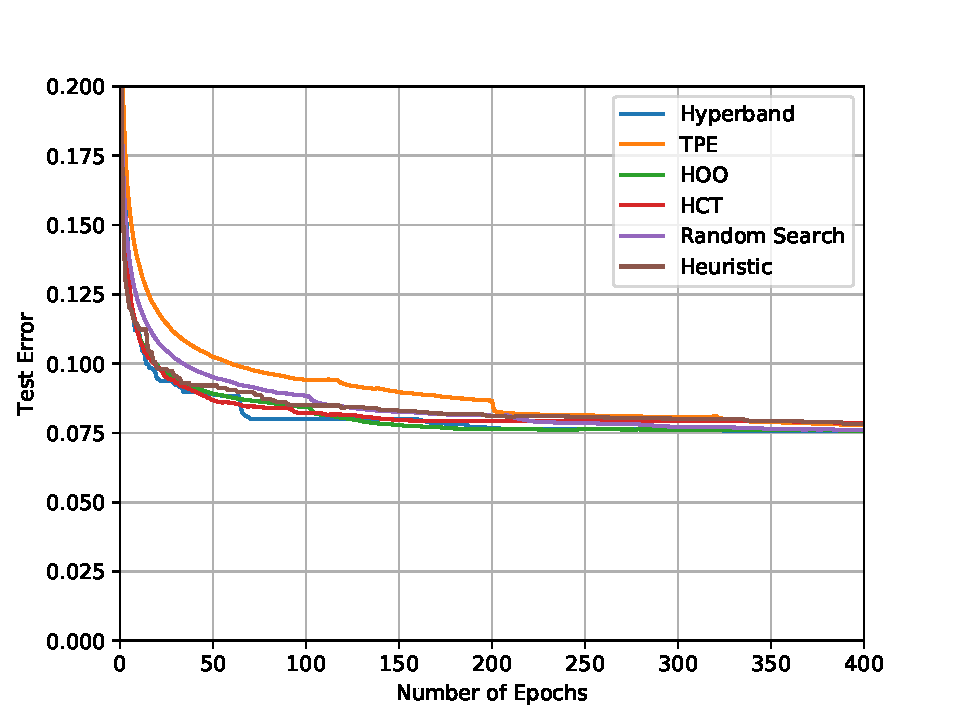
\includegraphics[width=5cm]{img/mnist/logistic_1.pdf} }}%
    \qquad
    \subfloat[\Hyperband and the heuristic]{{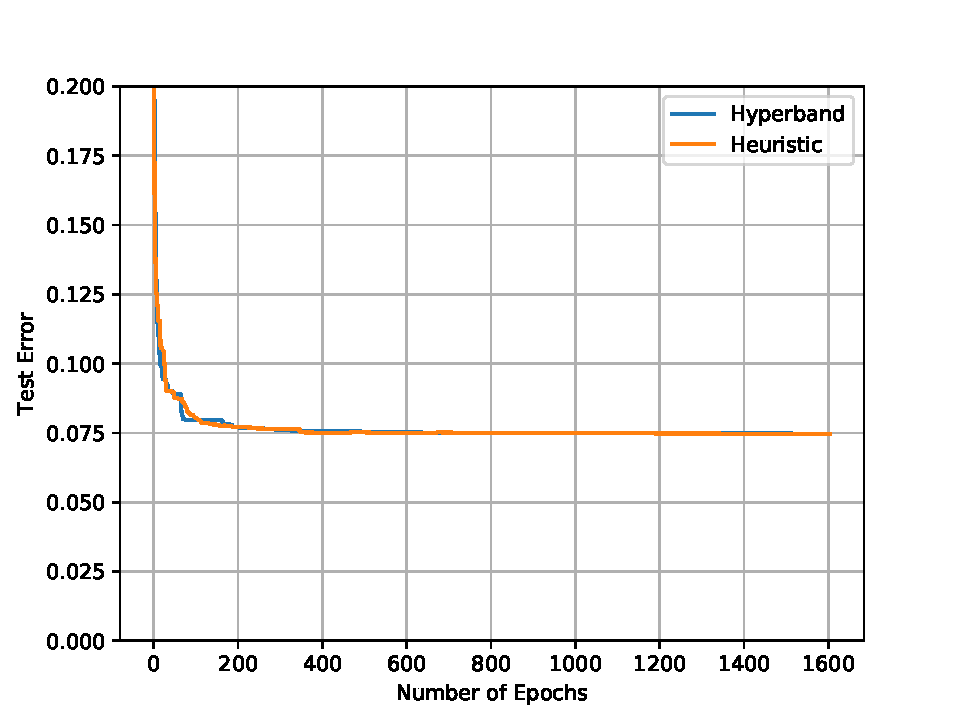
\includegraphics[width=5cm]{img/mnist/logistic_1_bis.pdf} }}%
    \caption{Comparing different hyper-parameter optimization algorithms on Logistic Regression, trained on \MNIST Dataset.}%
    \label{fig:logistic}%
\end{figure}

\begin{figure}[ht]
    \centering
    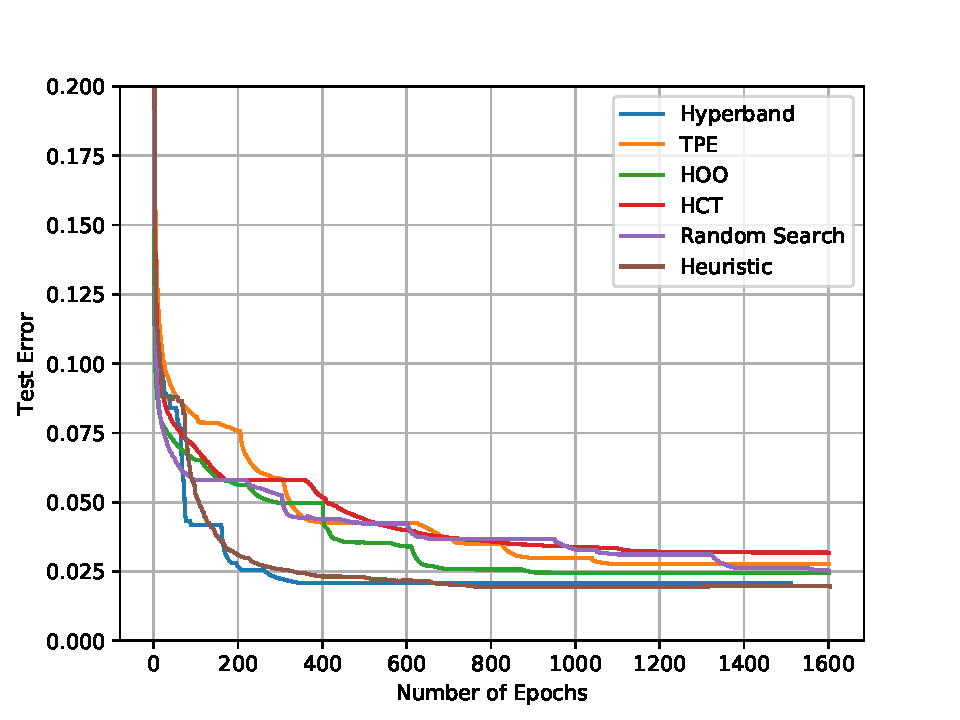
\includegraphics[scale=0.8]{img/mnist/mlp_0_bis.pdf}
    \caption{Comparing different hyper-parameter optimization algorithms on \MLP, trained on \MNIST Dataset.}
    \label{fig:mlp}
\end{figure}

\paragraph{\textbf{Discussion}} In the current setting, \Hyperband seems to be a plausible choice since it may explore more configurations compared to other algorithms. And comparing \Hyperband and the heuristic, we can see that they almost performs as well as each other. There are two major observations here. First, the heuristic seems to be converging more smoothly than \Hyperband, this is because \Hyperband focuses on evaluating one of the configurations after its round-robin tour among all the configurations in the bracket, which leads to a straight drop of the output loss. The second observation is that the heuristic seems to have a slightly better output at the end. This could be due to the fact that \TTTS is likely to evaluate the eventual best configuration more frequently than \SHA.


\subsection{Hyper-parameter tuning as SIAB problem}

We consider here Adaptive Boosting (AdaBoost), Gradient Boosting Machine (GBM), k-Nearest Neighbors (KNN), Multi-Layer Perceptron (\MLP), Support Vector Machine (SVM), Decision Tree and Random Forest from Scikit-learn.

\paragraph{\textbf{Dataset}} Several datasets on UCI dataset archive (e.g. Wine, Breast Cancer, etc) are being used. They are all pre-split into a training set $D_{\operatorname{train}}$ and a test set $D_{\operatorname{test}}$.

\paragraph{\textbf{Hyper-parameters}} The hyper-parameters to be optimized are listed below in Table \ref{adaparam}, \ref{gbmparam},  \ref{knnparam}, \ref{mlpparam}, \ref{svmparam}, \ref{treeparam} and \ref{rfparam}.

\begin{table}[ht]
\centering
\begin{tabular}{@{}lll@{}}
\toprule
\textbf{Parameter}             & \textbf{Type}  & \textbf{Bounds}                          \\ \midrule
\texttt{learning\_rate}      & $\mathbb{R}^+$ & $\left[10^{-5}, 10^{-1}\right]$                         \\
\texttt{n\_estimators}       & Integer        & $\left\lbrace 5,\dots, 200 \right\rbrace$
\end{tabular}
\caption{Hyper-parameters to be optimized for AdaBoost models.}
\label{adaparam}
\end{table}

\begin{table}[ht]
\centering
\begin{tabular}{@{}lll@{}}
\toprule
\textbf{Parameter}             & \textbf{Type}  & \textbf{Bounds}                          \\ \midrule
\texttt{learning\_rate}      & $\mathbb{R}^+$ & $\left[10^{-5}, 10^{-2}\right]$                         \\
\texttt{n\_estimators}       & Integer        & $\left\lbrace 10,\dots, 100 \right\rbrace$ \\
\texttt{max\_depth}          & Integer        & $\left\lbrace 2, \dots, 100 \right\rbrace$ \\
\texttt{min\_samples\_split}  & Integer        & $\left\lbrace 2, \dots, 100 \right\rbrace$
\end{tabular}
\caption{Hyper-parameters to be optimized for GBM models.}
\label{gbmparam}
\end{table}

\begin{table}[ht]
\centering
\begin{tabular}{@{}lll@{}}
\toprule
\textbf{Parameter} & \textbf{Type} & \textbf{Bounds}                           \\ \midrule
$k$                & Integer       & $\left\lbrace 10, \dots,50 \right\rbrace$
\end{tabular}
\caption{Hyper-parameters to be optimized for KNN models.}
\label{knnparam}
\end{table}

\begin{table}[ht]
\centering
\begin{tabular}{lll}
\hline
\textbf{Parameter}             & \textbf{Type}    & \textbf{Bounds}       \\ \hline
\texttt{hidden\_layer\_size} & Integer          & $\left[5, 50\right]$  \\
\texttt{alpha}               & $\mathbb{R}^{+}$ & $\left[0, 0.9\right]$
\end{tabular}
\caption{Hyper-parameters to be optimized for \MLP models.}
\label{mlpparam}
\end{table}

\begin{table}[ht]
\centering
\begin{tabular}{@{}lll@{}}
\toprule
\textbf{Parameter} & \textbf{Type}                      & \textbf{Bounds}               \\ \midrule
$C$                & $\mathbb{R}^+$ & $\left[ 10^{-5}, 10^{5} \right]$ (log-scaled) \\
$\gamma$           & $\mathbb{R}^+$ & $\left[10^{-5}, 10^{5} \right]$  (log-scaled)       \\ \bottomrule
\end{tabular}
\caption{Hyper-parameters to be optimized for SVM models.}
\label{svmparam}
\end{table}

\begin{table}[ht]
\centering
\begin{tabular}{@{}lll@{}}
\toprule
\textbf{Parameter}             & \textbf{Type}  & \textbf{Bounds}                          \\ \midrule
\texttt{max\_features}      & $\mathbb{R}^+$ & $\left[0.01, 0.99\right]$   \\
\texttt{max\_depth}          & Integer        & $\left\lbrace 4, \dots, 30 \right\rbrace$ \\
\texttt{min\_samples\_split}  & $\mathbb{R}^+$  & $\left[0.01, 0.99\right]$
\end{tabular}
\caption{Hyper-parameters to be optimized for Decision Tree models.}
\label{treeparam}
\end{table}

\begin{table}[ht]
\centering
\begin{tabular}{@{}lll@{}}
\toprule
\textbf{Parameter}             & \textbf{Type}  & \textbf{Bounds}                          \\ \midrule
\texttt{max\_features}      & $\mathbb{R}^+$ & $\left[0.1, 0.5\right]$   \\
\texttt{n\_estimators}          & Integer        & $\left\lbrace 10, \dots, 50 \right\rbrace$ \\
\texttt{min\_samples\_split}  & $\mathbb{R}^+$  & $\left[0.1, 0.5\right]$
\end{tabular}
\caption{Hyper-parameters to be optimized for Random Forest models.}
\label{rfparam}
\end{table}

\paragraph{\textbf{Resource Allocation}} One unit of resources in this setting is one iteration of training, which means one complete training of each classifier/regressor over the whole training set.

\paragraph{\textbf{Experimental Design}} In this section we use the logarithmic loss, also known as cross-entropy for classification problem, defined by:
\[
\ell(\theta, D) = - \frac{1}{|D|} \sum_{i=1}^{|D|} \sum_{j=1}^m y^{(i)}_{j}\log(\hat{p}^{(i)}_{j}),
\]
where $\hat{p}_{ij}$ is the predicted probability of a sample $i$ belonging to class $j$, and $m$ is the number of classes considered. And for regression problems, the loss that we use is the typical mean squared error, defined by:
\[
\ell(\theta, D) = - \frac{1}{|D|} \sum_{i=1}^{|D|} \left(y^{(i)} - \hat{y}^{(i)}_{\operatorname{pred}}\right)^2.
\]

And for this part of experiments, we choose to perform a shuffled $k=5$ cross-validation scheme on $D_{\operatorname{train}}$ at each time step $t$. In practice, this means that we fit $5$ models with the same architecture to different train/validation splits and average the loss results in each. More precisely, for every cross-validation split
$\mathtt{cv}_j,j=1\ldots5$, we get a loss $\ell_{j,t}(\hat{\theta}_{j,t}, D_{\operatorname{valid},j,t}) = \dfrac{1}{n} \sum^{n}_{i=1} \left(y^{(i)}_{j} - \hat{y}^{(i)}_{\operatorname{pred},j,t}\right)^2$, where $n=|D_{\operatorname{valid}}|$ (here we take MSE as an example, it's the same for log-loss). Thus the validation loss at time $t$ is
\[
\frac{1}{5}\sum_{j=1}^{5}\ell_{j,t}(\hat{\theta}_{j,t}, D_{\operatorname{valid},j,t}) = \frac{1}{5n}\sum_{j=1}^{5} \sum_{i=1}^n \left(y^{(i)}_{j} - \hat{y}^{(i)}_{\operatorname{pred},j,t}\right)^2.
\]
Just like in the previous section, we can then compute and report the test error on the holdout test set $D_{\operatorname{test}}$:
\[
\ell_{t}(\hat{\theta}_t, D_{\operatorname{test}}) = \frac{1}{|D_{\operatorname{test}}|} \sum_{i=1}^{|D_{\operatorname{test}}|} \left(y^{(i)} - \tilde{y}^{(i)}_{\operatorname{pred},t}\right)^2.
\]

Note that under this experimental environment, 'keep training' does not make sense anymore. Thus for HOO, TPE and Random Search, we only need to evaluate each configuration once, contrarily to what we did in the previous setting. While for Hyperband, we still need to evaluate each configuration for a certain times based on $R$ and $s_{\max}$.

\paragraph{\textbf{Comparison}} Each plot here is averaged on 20 runs of experiments. Fig.~\ref{fig:wine} displays the results for the Wine dataset, and Fig.~\ref{fig:breast_cancer} displays the results for the Brest Cancer dataset.

\begin{figure}%
    \centering
    \subfloat[\Ada]{{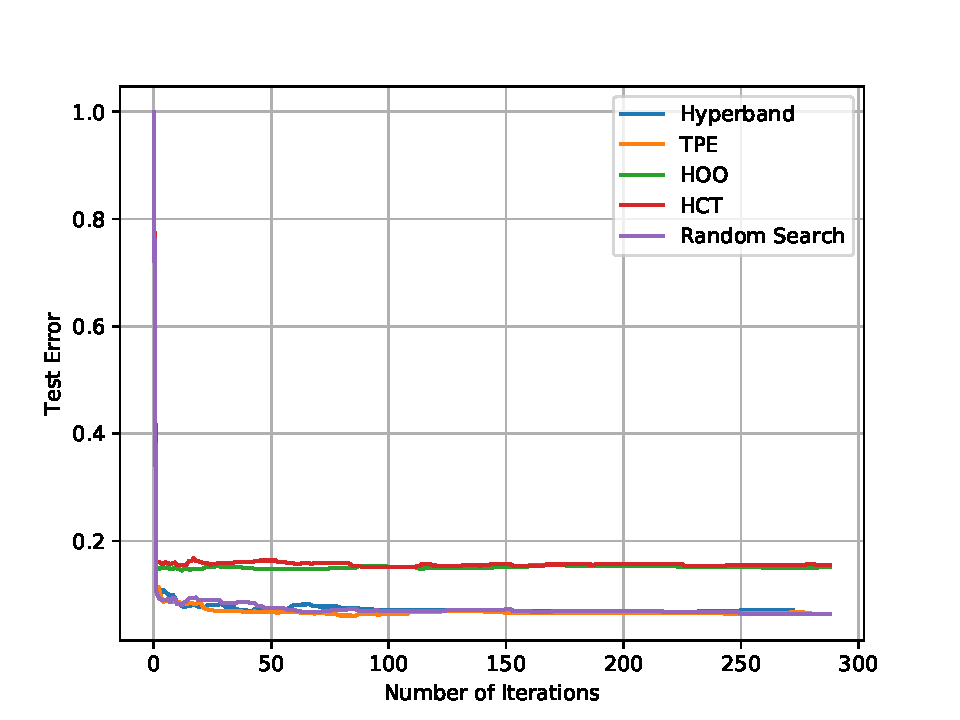
\includegraphics[width=5cm]{img/uci/ada_0.pdf} }}%
    \qquad
    \subfloat[\GBM]{{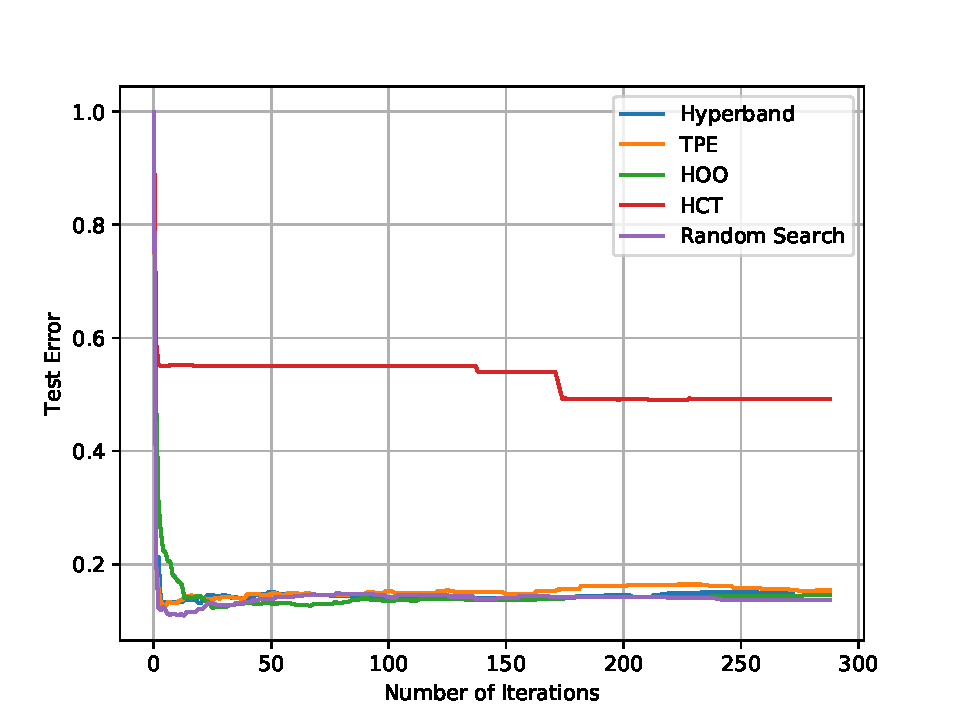
\includegraphics[width=5cm]{img/uci/gbm_0.pdf} }}%
    \qquad
    \subfloat[\KNN]{{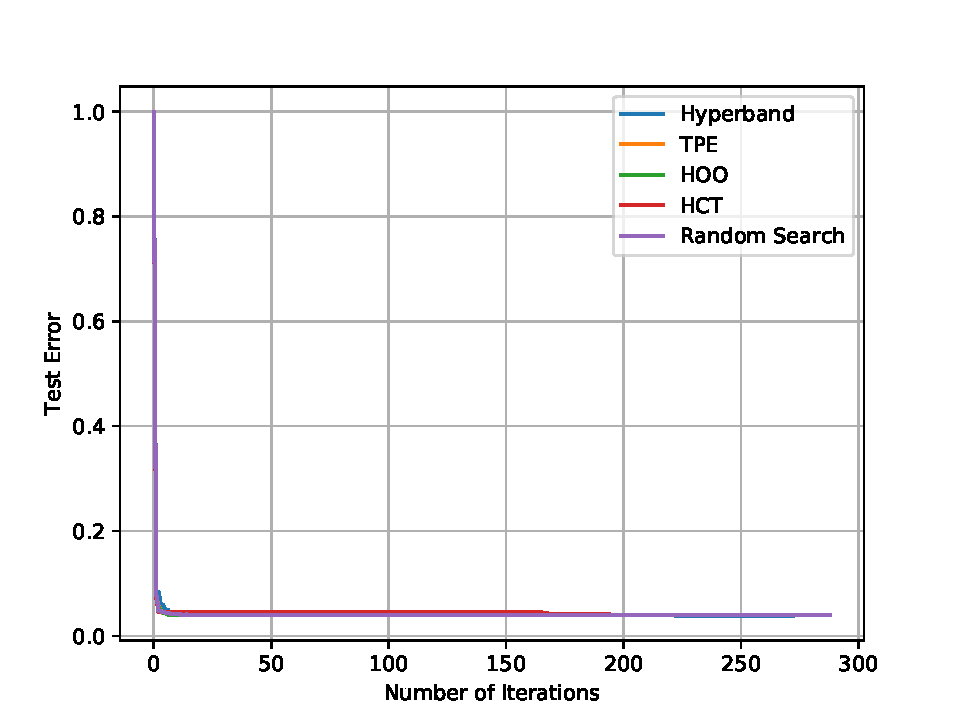
\includegraphics[width=5cm]{img/uci/knn_0.pdf} }}%
    \qquad
    \subfloat[\MLP]{{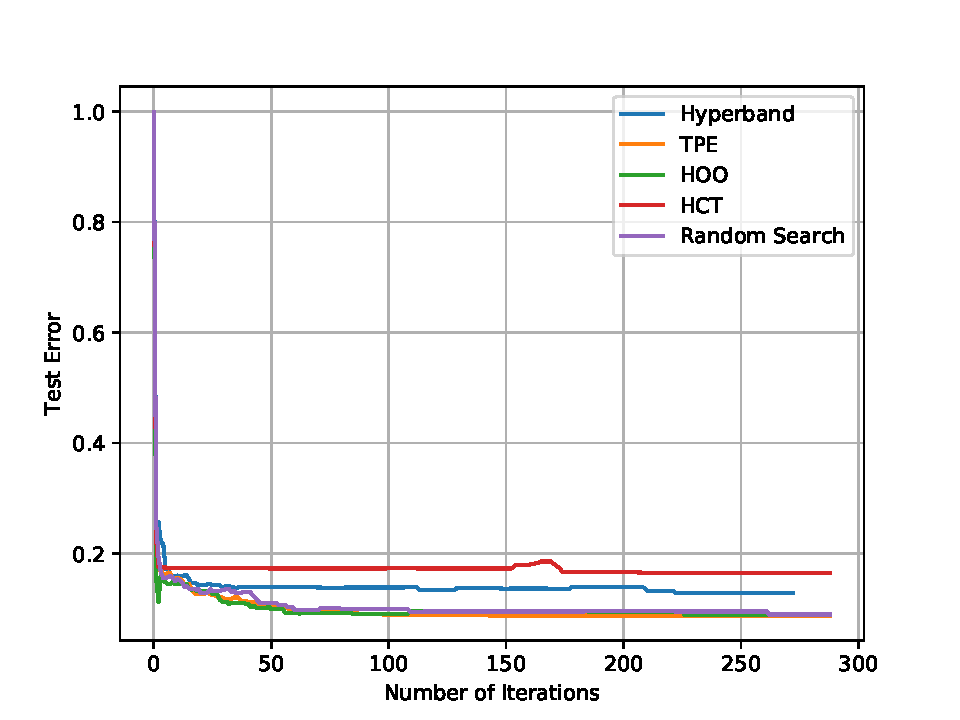
\includegraphics[width=5cm]{img/uci/sk_mlp_0.pdf} }}%
    \qquad
    \subfloat[\SVM]{{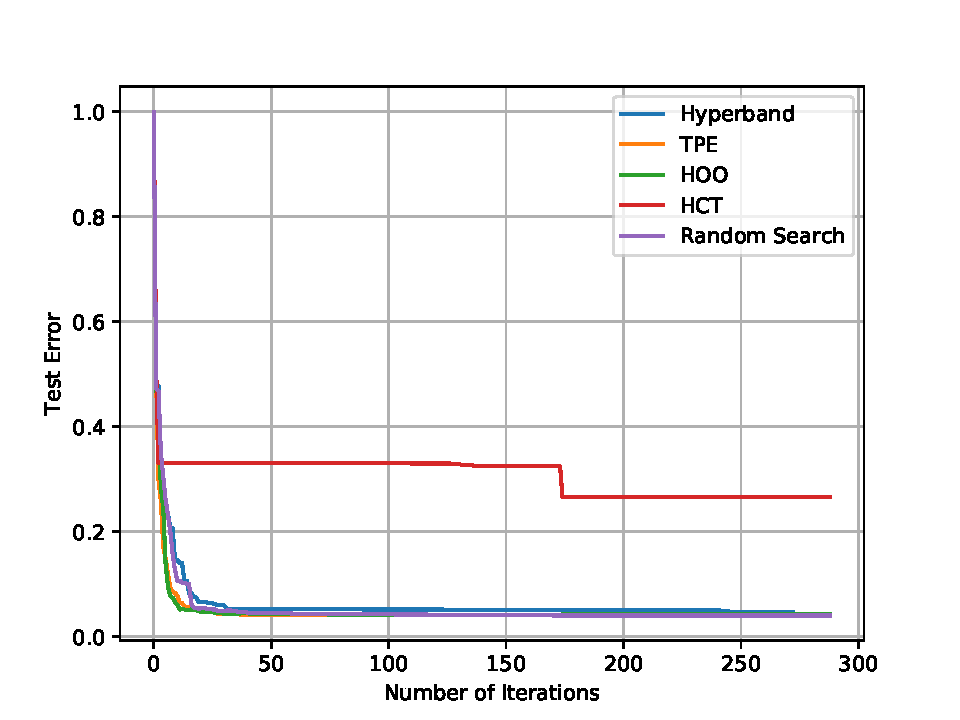
\includegraphics[width=5cm]{img/uci/svm_0.pdf} }}%
    \qquad
    \caption{Comparing different hyper-parameter optimization algorithms on different classifiers, trained on Wine dataset.}%
    \label{fig:wine}%
\end{figure}

\begin{figure}%
    \centering
    \subfloat[\Ada]{{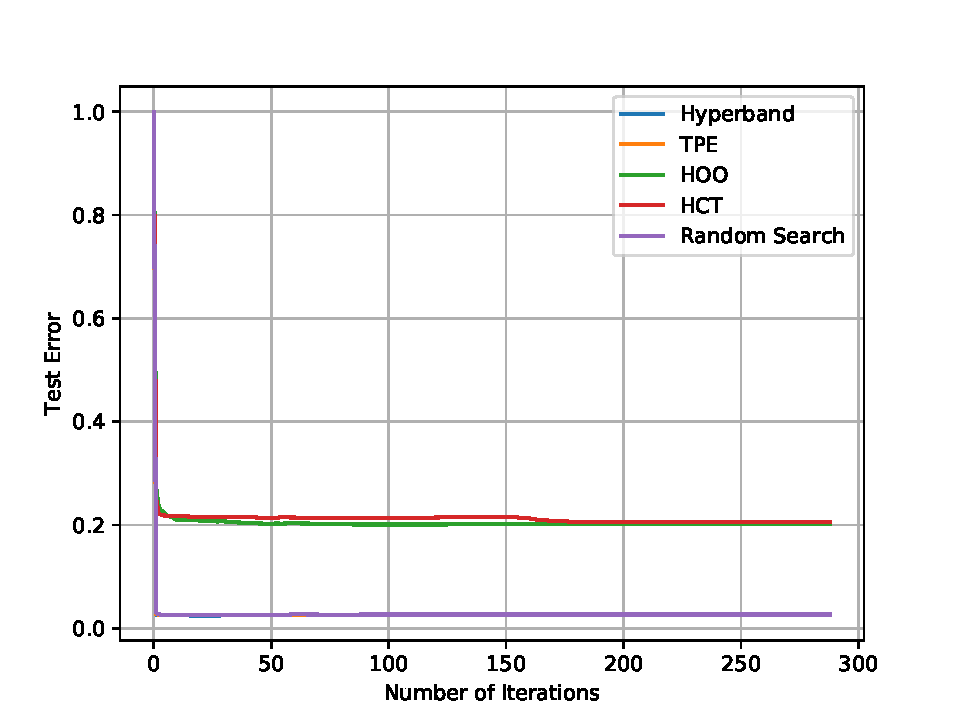
\includegraphics[width=5cm]{img/uci/ada_1.pdf} }}%
    \qquad
    \subfloat[\GBM]{{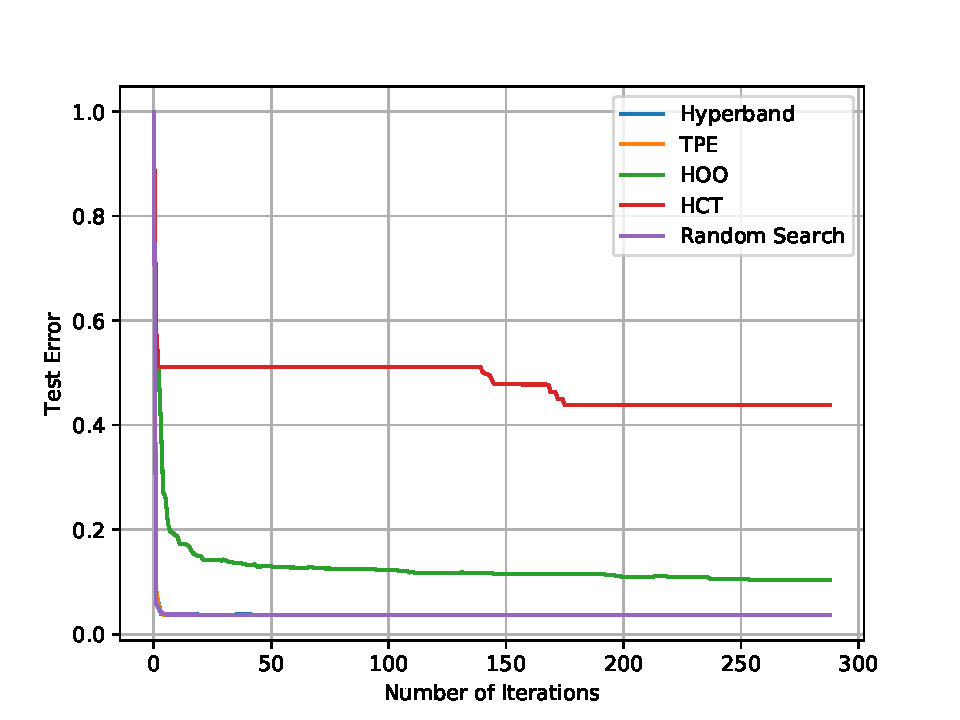
\includegraphics[width=5cm]{img/uci/gbm_1.pdf} }}%
    \qquad
    \subfloat[\KNN]{{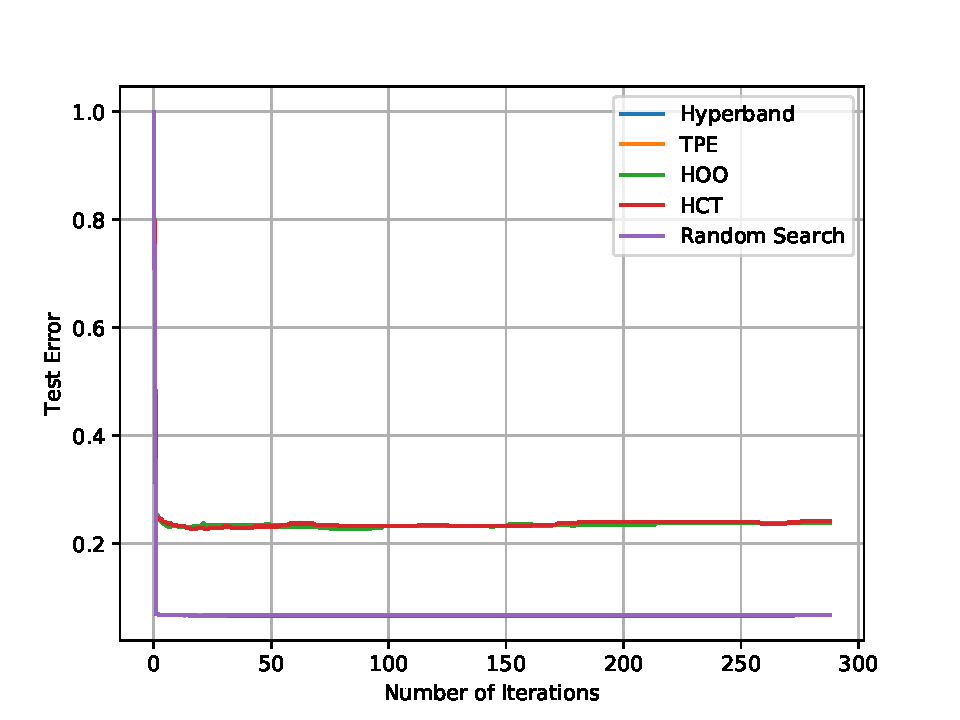
\includegraphics[width=5cm]{img/uci/knn_1.pdf} }}%
    \qquad
    \subfloat[\MLP]{{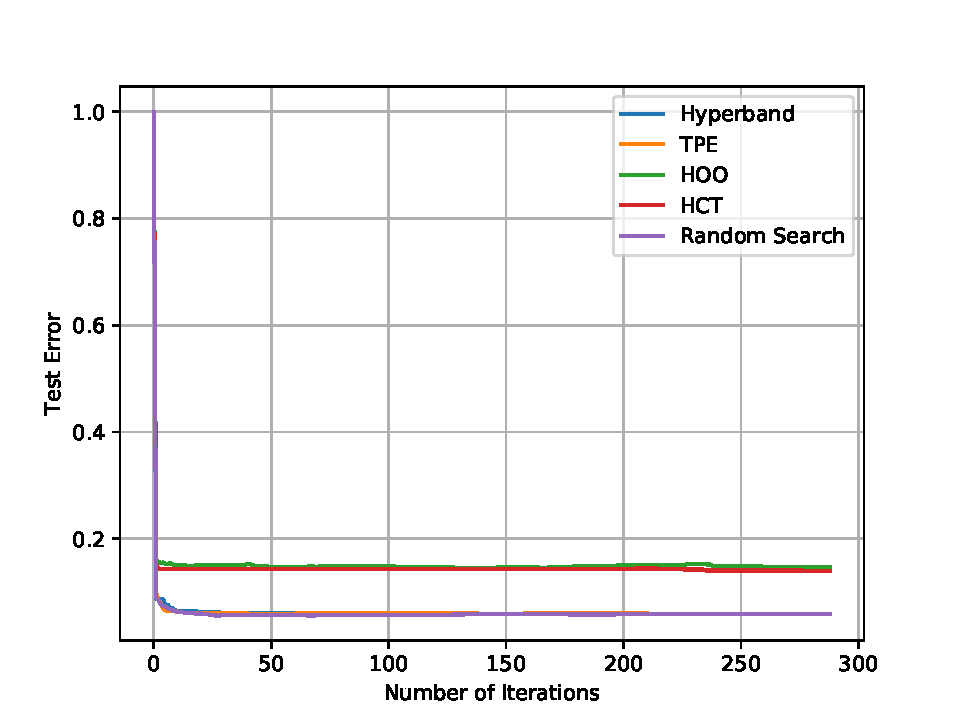
\includegraphics[width=5cm]{img/uci/sk_mlp_1.pdf} }}%
    \qquad
    \subfloat[\SVM]{{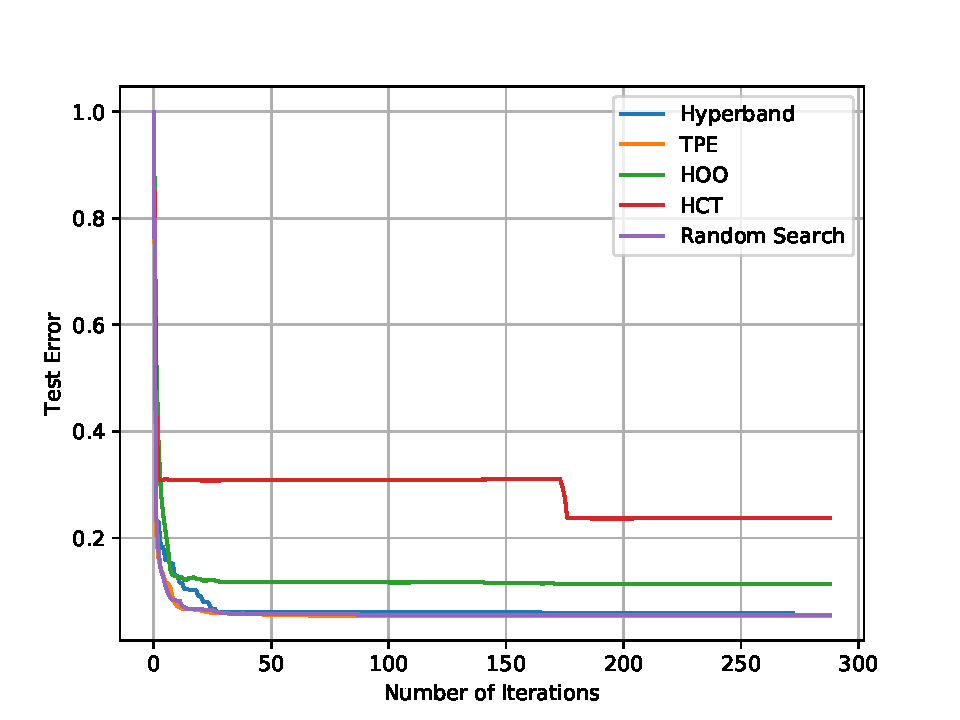
\includegraphics[width=5cm]{img/uci/svm_1.pdf} }}%
    \qquad
    \caption{Comparing different hyper-parameter optimization algorithms on different classifiers, trained on Breast Cancer dataset.}%
    \label{fig:breast_cancer}%
\end{figure}

\paragraph{\textbf{Discussion}} In this setting, Hyperband seems to loose its advantage of exploring more configurations. It appears to me that there is no reason for HOO, TPE and Random Search to evaluate one point several times as does Hyperband.

\newpage
\vskip 0.2in
\bibliography{Major}


%\section*{Appendix}

\end{document}
